\documentclass[sigconf]{acmart}

\setcopyright{none}
\setlength{\emergencystretch}{1em}
\acmConference[RecSys Challenge '26]{RecSys Challenge Workshop at ACM RecSys 2026}{September 2026}{Minneapolis, MN, USA}
\acmBooktitle{RecSys Challenge Workshop at ACM RecSys 2026, September 2026, Minneapolis, MN, USA}
\acmYear{2026}
\copyrightyear{2026}
\acmDOI{}
\acmISBN{}

% Auto-generated final devset selector.
\newcommand{\LocalEvaluationName}{Devset}
\newcommand{\LocalEvaluationRows}{8,000}
\newcommand{\LocalPreviewNotice}{}
\newcommand{\LocalScatterPath}{figures/retriever_recall_vs_size.pdf}
\newcommand{\RetrieverRowsFile}{generated_retriever_rows}
\newcommand{\FamilyRowsFile}{generated_family_rows}
% Generated by scripts/analyze_paper_results.py.
\newcommand{\DevRRFOne}{0.0605}
\newcommand{\DevRRFTen}{0.1502}
\newcommand{\DevRRFTwenty}{0.1715}
\newcommand{\DevNoProvOne}{0.0676}
\newcommand{\DevNoProvTen}{0.1610}
\newcommand{\DevNoProvTwenty}{0.1832}
\newcommand{\DevProvOnlyOne}{0.0709}
\newcommand{\DevProvOnlyTen}{0.1661}
\newcommand{\DevProvOnlyTwenty}{0.1869}
\newcommand{\DevNoTpdOne}{0.0761}
\newcommand{\DevNoTpdTen}{0.1765}
\newcommand{\DevNoTpdTwenty}{0.1989}
\newcommand{\DevFullOne}{0.0770}
\newcommand{\DevFullTen}{0.1769}
\newcommand{\DevFullTwenty}{0.1994}
\newcommand{\DevUnionRecallAll}{0.7186}
\newcommand{\DevUnionMeanCandidates}{790.1}
\newcommand{\DevBMRecallAll}{0.4990}
\newcommand{\DevTwoTowerRecallAll}{0.4860}
\newcommand{\DevTwoTowerUniqueHits}{540}
\newcommand{\DevBMUniqueHits}{178}
\newcommand{\DevTrackCoocUniqueHits}{176}
\newcommand{\DevSemanticAblation}{0.0675}
\newcommand{\DevLexicalAblation}{0.0554}
\newcommand{\DevBehavioralAblation}{0.0517}
\newcommand{\RetrievalMissLoss}{0.2814}
\newcommand{\RerankMissLoss}{0.3275}
\newcommand{\OrderingLoss}{0.1917}
\newcommand{\RetrievalMissRows}{2,251}
\newcommand{\RerankMissRows}{2,620}
\newcommand{\OrderingLossRows}{2,513}
\newcommand{\DevRRFMinTwenty}{0.1706}
\newcommand{\DevRRFMaxTwenty}{0.1738}
\newcommand{\DevFullVsRRFGain}{0.0279}
\newcommand{\DevPerRetrieverFeatureGain}{0.0162}
\newcommand{\DevTpdRecallGain}{0.0159}
\newcommand{\DevTpdNDCGGain}{0.0005}



\title[Multi-Source Conversational Music Recommendation]{%
  A Practical Multi-Source Pipeline for Conversational Music Recommendation
  in the RecSys Challenge 2026}

\author{Ryohei Wakatsuki}
\email{r.wakatsuki1207@gmail.com}
\affiliation{%
  \institution{Independent Researcher}
  \city{Tokyo}
  \country{Japan}}

\begin{abstract}
Our submission under the team name \textit{niwatori} ranked third overall in
the RecSys Challenge 2026 Music-CRS task.  The pipeline combines candidates from
14 retrieval sources while retaining, for each candidate, which sources
returned it and their ranks and scores.
It uses these signals together with context--track features in a LightGBM
LambdaRank reranker.  A Qwen3.6-27B responder verbalizes the top ranked tracks.
The submission also ranked third in nDCG@20 on the final Blind-B leaderboard.
We complement the leaderboard result with a diagnostic that fits on Train and
evaluates the official Devset.  In this diagnostic, we compare the full pipeline
with reciprocal-rank fusion, ablate per-retriever features, and
decompose ranking error into retrieval misses, reranking exclusions, and
ranks-2--20 ordering loss.  Code is
available at \url{https://github.com/ryowk/recsys2026-niwatori}.
\end{abstract}

\ccsdesc[500]{Information systems~Recommender systems}
\ccsdesc[300]{Information systems~Learning to rank}
\keywords{conversational recommendation, music recommendation, multi-source retrieval, learning to rank}

\begin{document}
\maketitle

\section{Introduction}
Conversational music recommendation must reconcile signals at different
granularities: an exact title request, a mood expressed in natural language,
entities and reactions in previous turns, and behavioral relations among
tracks.  A single retriever is unlikely to cover all these cases.  Conversely,
reducing outputs from multiple retrievers to one hand-tuned score discards
which retriever returned a candidate and how confidently it did so.

Our RecSys Challenge 2026 pipeline addresses this practical problem with a wide
candidate union followed by LambdaRank reranking.  It keeps per-source
presence, rank, and score signals rather than treating retrieval only as a
set-valued preprocessing step.  We make three contributions: (1) a reproducible 14-source retrieval
pipeline spanning lexical, semantic, entity/history, and sequential signals;
(2) a LambdaRank reranker that combines per-retriever features with independently
computed context--track features; and (3) component-wise analysis of source
complementarity, a reciprocal-rank fusion (RRF) baseline, and ranking-error
decomposition.  We do not
claim a new ranking algorithm; the contribution is an empirically analyzed
pipeline design under competition constraints.  This follows the broader view
of conversational recommenders as systems that jointly elicit preferences and
select items over multiple turns~\cite{jannach2021survey}.

\section{Task and Evaluation Protocol}
Music-CRS evaluates one target at each $(\mathit{session\_id},
\mathit{turn\_number})$ pair~\cite{challenge2026}.  The system observes the
current user utterance and preceding dialogue, together with user context when
available; track metadata and organizer-provided track/user embeddings are
also supplied.  It must retrieve from the entire 47,071-track catalog, return
20 ranked track identifiers, and generate a natural-language response that
accompanies and explains the recommendations.

The ranked list and generated response are evaluated with four metrics.
For ranking, nDCG@20 measures the position of the ground-truth track, while
catalog diversity measures the
fraction of catalog tracks recommended across all evaluated lists.  Each
target has one ground-truth track, so nDCG@20 is $1/\log_2(r+1)$ when it appears
at rank $r\leq20$, and zero otherwise.  For the responses, Distinct-2 is the
number of unique bigrams divided by the total number of bigrams across all
responses, and a 1--5 LLM judge scores personalization and explanation
quality.  The composite score is their weighted average:
$0.50\,\mathrm{nDCG@20}+0.10\,\mathrm{CatalogDiv}+0.10\,\mathrm{Distinct2}
+0.30\,(\mathrm{Judge}-1)/4$.
Table~\ref{tab:blind} reports the official Blind-B scores.

The public labeled data contain 16,199 eight-turn conversations (129,592
targets).  We call the 15,199-conversation split (121,592 targets) \emph{Train}
and the official 1,000-conversation split (8,000 targets) \emph{Devset}.
Challenge-time development used five-fold cross-validation (CV) over
Train$+$Devset, and the final Blind-B pipeline was fit on that public pool.
For the paper analysis, we instead fit on Train and evaluate Devset once;
because Devset influenced earlier development, this is a diagnostic rather
than an independent test result.
Blind B contains 80 evaluated targets and includes cold-start cases in which
user identity and profile are unavailable.

Retrievers that use training labels produce out-of-fold (OOF) features: each
Train row is processed by a retriever fitted without its fold.  These features
train one reranker; retrievers fitted on all of Train generate Devset candidates.
Figure~\ref{fig:pipeline} shows the analogous submitted procedure.  Locally, we
report retriever Recall@20, Recall@all, Precision@all, emitted-candidate count,
and unique gold hits.  Ranking metrics are nDCG@1/10/20.

\begin{figure*}[t]
  \centering
  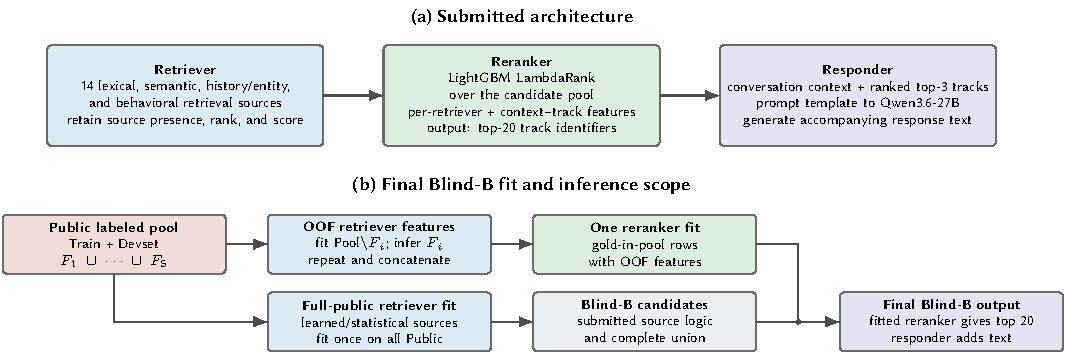
\includegraphics[width=\textwidth]{figures/pipeline.pdf}
  \caption{Submitted pipeline and Blind-B fit scope. Five-fold out-of-fold
  (OOF) retriever features train one reranker. Retrievers fitted on the public
  pool supply Blind-B candidates; fit-free retrievers require no fold-specific model.}
  \Description{The upper panel shows Retriever, Reranker, and Responder blocks with their inputs and outputs. The lower panel shows public labeled data split into five folds, out-of-fold retriever feature construction for one reranker fit, and full-public retriever inference on Blind B.}
  \label{fig:pipeline}
\end{figure*}

\begin{table}[t]
  \caption{Official Blind-B leaderboard scores for \textit{niwatori}.}
  \label{tab:blind}
  \centering
  \small
  \begin{tabular}{lr}
    \toprule
    Metric & Score \\
    \midrule
    \textbf{Composite score} & \textbf{0.5859} \\
    \midrule
    nDCG@20 & 0.4934 \\
    Catalog diversity & 0.0312 \\
    Lexical diversity (Distinct-2) & 0.7736 \\
    LLM judge & 4.45 \\
    \bottomrule
  \end{tabular}
\end{table}

\section{Method}
\subsection{Multi-source candidate retrieval}
For every turn, all 14 retrievers search the full challenge catalog, as required
by the task~\cite{challenge2026}.  BM25~\cite{robertson2009bm25} and TF--IDF compare the current message
and observed dialogue context with track metadata.  Tag-intent retrieval
searches catalog tags using detected genre, mood, and descriptor terms, while
exact title/artist and album/artist sources expand explicit entity mentions.
The supervised two-tower learns dense query--track similarity with a
LoRA-adapted Qwen3-Embedding-0.6B query tower~\cite{hu2022lora,qwen3embedding}.
History-artist and history-album expand entities from all previously observed
tracks; last-artist and last-album use only the latest music turn.  Track
co-occurrence aggregates neighbors of all history tracks, last-track
transition predicts the next track, and album/artist co-occurrence applies the
same neighborhood signal at coarser entity levels.

Sources return broad ranked lists with their raw and auxiliary scores.  The
submission configuration applies source-specific caps: 200 each for BM25,
TF--IDF, and two-tower; 100 for tag intent; and 500/200/100 for
track/album/artist co-occurrence.  These settings bound reranking cost and were
not exhaustively tuned.  Uncapped sources contribute their full stored lists.
Album co-occurrence additionally requires count $\geq 5$.  We concatenate the
lists and collapse duplicate IDs while retaining every source's features; no
global cap then truncates the union.
Every candidate retains whether each retriever returned it, its within-retriever
rank and score, the number of supporting retrievers, and best/mean retriever
rank.  We refer to these directly as per-retriever features.

We used two public external datasets in limited roles.  Mapped track sequences from
TalkPlayData-1 (TPD1)~\cite{talkplay,tpd1card} augment only co-occurrence
and transition counts.
TalkPlayData-2~\cite{talkplaydata2} is
used only for catalog ID mapping.

\subsection{LambdaRank reranking with per-retriever features}
The reranker processes the complete union and outputs 20 tracks.  It is a
LightGBM LambdaRank model~\cite{burges2010lambdamart,ke2017lightgbm}.  Its
features fall into two groups.  Per-retriever features encode source presence,
within-source ranks and transformations, and raw/normalized scores.  They also
include source-overlap summaries, such as how many retrievers returned a candidate.
Context--track features are computed independently of source outputs and encode
query--metadata and dense similarity,
history consistency, artist/album/tag relations, duration and release
metadata, and hierarchical popularity.  Training keeps only rows whose gold
track occurs in the candidate pool; this reproduces the final pipeline's
gold-in-pool training rule.

For the paper evaluation, we preserve the submitted OOF/full-fit roles shown
in Figure~\ref{fig:pipeline}, replacing the public pool with Train and Blind B
with Devset.  Thus no Devset row or label enters retriever or reranker
fitting; fit-free retrievers require no fold model.

\subsection{Response generation}
\label{sec:response-generation}
Figure~\ref{fig:responder-example} illustrates how a fixed prompt template grounds
a submitted response in the current request and ranked track metadata.
\begin{figure*}[!t]
  \centering
  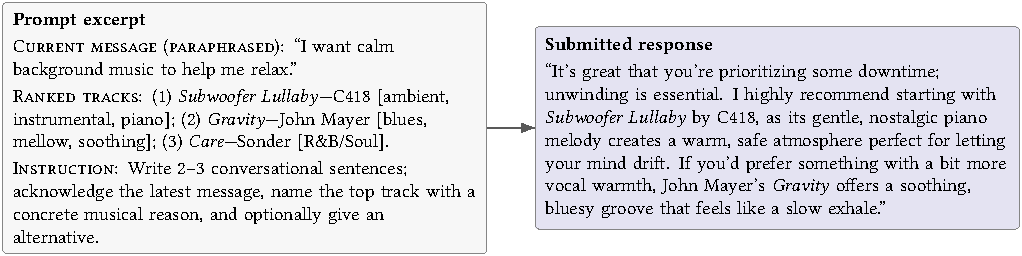
\includegraphics[width=\textwidth]{figures/responder_example.pdf}
  \caption{Cold-start Blind-B example with a paraphrased request, the actual
  ranked tracks, and the verbatim Qwen3.6-27B response selected for the final
  submission.  The complete template also contains reusable role instructions
  and optional context blocks; profile and conversation history are empty in
  this row.}
  \Description{The left box shows a relaxation request, three ranked tracks with metadata, and response constraints. An arrow points to the generated natural-language recommendation in the right box.}
  \label{fig:responder-example}
\end{figure*}

The top-3 reranked tracks, available user/profile fields, conversation
history, and current message are inserted into a fixed prompt template and
passed to Qwen3.6-27B~\cite{qwen36model}.  Generation uses 200 output tokens,
temperature 0.7, and top-$p$ 0.9, with thinking disabled.  The prompt asks for
two or three sentences that acknowledge the latest message, name the first
track with a concrete musical reason and optionally mention an alternative.
The responder generates only the accompanying text; ranking is completed
upstream.  The final submission generated ten seeded responses per Blind-B row.
We selected one candidate per row using a corpus-level lexical-diversity proxy.
This step changes only response text; it is an output-selection procedure rather
than a responder-model contribution.

\section{Results and Analysis}
\LocalPreviewNotice
The submission ranked third overall and on nDCG@20.  Blind B contains ten rows
at each turn 1--8
and withholds user identity and profile for 40 of its 80 rows.  Its absolute
nDCG is therefore not treated as directly comparable with the 8,000-row
Devset result.

\paragraph{Response selection.}
For a direct comparison of the selection step in
Section~\ref{sec:response-generation}, we recomputed Distinct-2 from the
submitted response set and the ten underlying single-run outputs.  The
single-run outputs averaged 0.7217 (best 0.7287), while selection increased
Distinct-2 to 0.7736.

\subsection{Retriever complementarity}
\begin{table*}[t]
  \caption{Submitted-source metrics on \LocalEvaluationName. Recall@all is the
  fraction of targets whose gold track appears anywhere in the source's
  candidates; Delta Recall@all is the drop in union Recall@all when that source
  is removed. nDCG@20 averages within source-score ties, and Unique gold hits
  counts targets retrieved by that source and no other.}
  \label{tab:retrievers}
  \centering
  \scriptsize
  \setlength{\tabcolsep}{2.3pt}
  \begin{tabular}{@{}llrrrrrrr@{}}
    \toprule
    Source & Family & \shortstack{Mean\\candidates} & nDCG@20 &
    Recall@20 & Recall@all & Precision@all & \shortstack{Unique gold\\hits} &
    \shortstack{Delta\\Recall@all} \\
    \midrule
    \input{\RetrieverRowsFile}
  \end{tabular}
\end{table*}

\begin{table*}[t]
  \centering
  \begin{minipage}[t]{0.42\textwidth}
    \caption{Family complementarity on \LocalEvaluationName. Metrics follow
    Table~\ref{tab:retrievers}, treating each family as the retrieval unit.}
    \label{tab:families}
    \centering
    \footnotesize
    \setlength{\tabcolsep}{3.6pt}
    \begin{tabular}{@{}lrrr@{}}
      \toprule
      Family & Recall@all & \shortstack{Unique gold\\hits} & \shortstack{Delta\\Recall@all} \\
      \midrule
      \input{\FamilyRowsFile}
    \end{tabular}
  \end{minipage}\hfill
  \begin{minipage}[t]{0.55\textwidth}
    \caption{Local ranking results on \LocalEvaluationName. Values are
    descriptive means over \LocalEvaluationRows{} rows.}
    \label{tab:ablation}
    \centering
    \footnotesize
    \setlength{\tabcolsep}{3.4pt}
    \begin{tabular}{@{}lrrr@{}}
      \toprule
      Ranker & nDCG@1 & nDCG@10 & nDCG@20 \\
      \midrule
      Tie-aware RRF ($k=60$) & \DevRRFOne & \DevRRFTen & \DevRRFTwenty \\
      \addlinespace[2pt]
      \multicolumn{4}{l}{\itshape LambdaRank variants} \\
      Context--track only & \DevNoProvOne & \DevNoProvTen & \DevNoProvTwenty \\
      Per-retriever only & \DevProvOnlyOne & \DevProvOnlyTen & \DevProvOnlyTwenty \\
      Full, without TPD1 & \DevNoTpdOne & \DevNoTpdTen & \DevNoTpdTwenty \\
      Full & \textbf{\DevFullOne} & \textbf{\DevFullTen} & \textbf{\DevFullTwenty} \\
      \bottomrule
    \end{tabular}
  \end{minipage}
\end{table*}

\begin{figure}[t]
  \centering
  \IfFileExists{\LocalScatterPath}{%
    \includegraphics[width=\columnwidth]{\LocalScatterPath}%
  }{\fbox{\parbox[c][0.19\textheight][c]{0.92\columnwidth}{\centering Devset retriever plot pending}}}
  \caption{Submitted-source Recall@all versus mean candidate count on
  \LocalEvaluationName{} (logarithmic horizontal axis).}
  \Description{Scatter plot of recall against mean emitted candidates, colored by retriever family, with the complete union highlighted.}
  \label{fig:retrievers}
\end{figure}

Figure~\ref{fig:retrievers} plots each submitted source's coverage against its
candidate volume, while Table~\ref{tab:retrievers} reports source-level ranking
and coverage statistics.  The union reaches \DevUnionRecallAll\ Recall@all with
\DevUnionMeanCandidates\ mean candidates.  BM25, the best standalone source,
reaches \DevBMRecallAll, and the two-tower reaches \DevTwoTowerRecallAll.  The
sources provide complementary coverage:
the two-tower finds \DevTwoTowerUniqueHits{} gold tracks missed by every other
source, while BM25 and track co-occurrence contribute \DevBMUniqueHits{} and
\DevTrackCoocUniqueHits{} such unique hits, respectively.

Table~\ref{tab:families} groups the sources by signal family and measures each
family's unique coverage and the union's loss when that family is removed.
Removing the semantic, lexical, or behavioral family lowers union Recall@all by
\DevSemanticAblation, \DevLexicalAblation, and \DevBehavioralAblation,
respectively.
A zero in Unique gold hits means only that a source does not expand gold coverage
beyond the other sources on this Devset.  It can still help rank candidates
also found elsewhere through its presence, rank, and score features, or add
coverage on another split.  Zero unique coverage therefore does not imply that
the source should be removed.

\subsection{Fusion and per-retriever features}
Table~\ref{tab:ablation} compares controlled LambdaRank variants with
reciprocal-rank fusion (RRF)~\cite{cormack2009rrf}, a non-learned baseline over
the same complete union.  Our tie-aware RRF uses $k=60$ and assigns equal
within-source scores their average rank.  In \emph{Context--track only}, we
remove all source-derived columns.  In
\emph{Per-retriever only}, we retain source presence, ranks, scores, and overlap
summaries.  \emph{Full} combines the two feature groups.  The three LambdaRank
feature variants use the same candidates, training rows, and parameters.
\emph{Full, without TPD1} instead rebuilds the track co-occurrence and
transition sources without external counts, making it an external-data
ablation.

RRF reaches \DevRRFTwenty.  The reported baseline uses $k=60$, fixed before
this Devset analysis.  Across $k\in\{10,30,60,100\}$, nDCG@20 spans
\DevRRFMinTwenty--\DevRRFMaxTwenty.
The full LambdaRank reranks the same complete union and reaches
\DevFullTwenty, improving nDCG@20 by \DevFullVsRRFGain{} over RRF.

The feature ablations show how this gain is obtained.  Context--track features
alone reach \DevNoProvTwenty, and per-retriever features alone reach
\DevProvOnlyTwenty.  Combining both groups reaches \DevFullTwenty, a
\DevPerRetrieverFeatureGain{} improvement over context--track features alone.
The external sequences have a smaller downstream effect: TPD1 raises union
Recall@all by \DevTpdRecallGain, while nDCG@20 increases by only
\DevTpdNDCGGain.

\subsection{Error decomposition}
We attribute each row's nDCG shortfall to one stage.  A \emph{retrieval miss}
means the gold track is absent from the union; a \emph{reranking exclusion}
means it is retrieved but remains outside the top 20; and \emph{ordering loss}
is its remaining discount at ranks 2--20.

Reranking exclusion is the largest component
(\RerankMissLoss; \RerankMissRows{} of \LocalEvaluationRows{} rows), followed
by retrieval misses (\RetrievalMissLoss; \RetrievalMissRows{} rows) and
ordering at ranks 2--20 (\OrderingLoss; \OrderingLossRows{} rows).  These
cases are mutually exclusive, and their mean losses sum to
$1-\mathrm{nDCG@20}$.  The main opportunity is therefore to move
already-retrieved gold tracks into the top 20, while continuing to expand
candidate coverage.

\section{Limitations and Conclusion}
Blind B contains only 80 hidden-label rows, so its absolute nDCG is not directly
comparable with Devset.  Without its hidden labels, we cannot attribute the
score difference to a particular cause.  Local evaluation also cannot
reproduce the LLM judge.

Within these limits, our main result is a practical end-to-end recipe rather
than a new ranking algorithm: search the full catalog with heterogeneous
retrievers, preserve their provenance instead of collapsing them into one
heuristic score, learn a single reranker on leak-controlled OOF features, and
verbalize its ranked output without changing the recommendation list.  This
pipeline ranked third overall and on nDCG@20.  The Devset analysis explains both
why it works---the union expands coverage and per-retriever features improve
nDCG@20 by \DevPerRetrieverFeatureGain---and its main remaining weakness:
reranking exclusion.  More broadly, reusable lessons include using
heterogeneous retrievers to expand coverage and retaining source-specific
evidence after candidate generation as input to learned ranking.

\clearpage
\bibliographystyle{ACM-Reference-Format}
\bibliography{references}
\end{document}
